\documentclass[border=10pt]{standalone}
\usepackage{tikz}
\usepackage{tikz-uml}

\begin{document}

\begin{tikzpicture}
% ============================================================================
% Core Object Classes
% ============================================================================

% PoseObjectPNP - Position and Orientation
\umlclass[x=0.5, y=2]{PoseObjectPNP}{
  + x : float \\
  + y : float \\
  + z : float \\
  + roll : float \\
  + pitch : float \\
  + yaw : float
}{
  + \_\_init\_\_(x, y, z, roll, pitch, yaw) \\
  + \_\_add\_\_(other) : PoseObjectPNP \\
  + \_\_sub\_\_(other) : PoseObjectPNP \\
  + \_\_eq\_\_(other) : bool \\
  + approx\_eq(other, eps\_position, eps\_orientation) : bool \\
  + approx\_eq\_xyz(other, eps) : bool \\
  + copy\_with\_offsets(...) : PoseObjectPNP \\
  + to\_list() : List[float] \\
  + to\_transformation\_matrix() : ndarray \\
  + xy\_coordinate() : List[float] \\
  + quaternion : List[float] \{property\} \\
  + quaternion\_pose : List[float] \{property\} \\
  + \{static\} euler\_to\_quaternion(...) : List[float] \\
  + \{static\} quaternion\_to\_euler\_angle(...) : Tuple
}

% ObjectAPI - Abstract Interface
\umlclass[x=11, y=-11]{ObjectAPI}{
  \{abstract\}
}{
  + \{abstract\} label() : str \\
  + \{abstract\} coordinate() : List[float]
}

% Location Enum
\umlclass[x=11, y=4.1]{Location}{
  LEFT\_NEXT\_TO \\
  RIGHT\_NEXT\_TO \\
  ABOVE \\
  BELOW \\
  ON\_TOP\_OF \\
  INSIDE \\
  CLOSE\_TO \\
  NONE
}{
  + \{static\} convert\_str2location(location) : Location
}

% Object - Detected Object
\umlclass[x=0.5, y=-11]{Object}{
  - \_label : str \\
  - \_workspace : Workspace \\
  - \_pose\_center : PoseObjectPNP \\
  - \_pose\_com : PoseObjectPNP \\
  - \_width\_m : float \\
  - \_height\_m : float \\
  - \_size\_m2 : float \\
  - \_gripper\_rotation : float \\
  - \_largest\_contour : ndarray \\
  - \_verbose : bool
}{
  + \_\_init\_\_(label, u\_min, v\_min, u\_max, v\_max, mask\_8u, workspace) \\
  + label() : str \\
  + coordinate() : List[float] \\
  + xy\_com() : Tuple[float, float] \\
  + xy\_center() : Tuple[float, float] \\
  + pose\_center() : PoseObjectPNP \\
  + pose\_com() : PoseObjectPNP \\
  + shape\_m() : Tuple[float, float] \\
  + width\_m() : float \\
  + height\_m() : float \\
  + size\_m2() : float \\
  + gripper\_rotation() : float \\
  + workspace() : Workspace \\
  + to\_dict() : Dict \\
  + to\_json() : str \\
  + \{static\} from\_dict(data, workspace) : Object \\
  + \{static\} from\_json(json\_str, workspace) : Object \\
  + as\_string\_for\_llm() : str \\
  + as\_string\_for\_chat\_window() : str \\
  + \{static\} calc\_width\_height(pose\_ul, pose\_lr) : Tuple
}

% Objects - Collection
\umlclass[x=13, y=-3]{Objects}{
  - \_verbose : bool
}{
  + \_\_init\_\_(iterable, verbose) \\
  + get\_detected\_object(coordinate, label) : Object \\
  + get\_detected\_objects(location, coordinate, label) : Objects \\
  + get\_nearest\_detected\_object(coordinate, label) : Tuple \\
  + get\_largest\_detected\_object() : Tuple \\
  + get\_smallest\_detected\_object() : Tuple \\
  + get\_detected\_objects\_sorted(ascending) : Objects \\
  + get\_detected\_objects\_as\_comma\_separated\_string() : str \\
  + \{static\} objects\_to\_dict\_list(objects) : List[Dict] \\
  + \{static\} dict\_list\_to\_objects(dict\_list, workspace) : Objects
}

% ============================================================================
% Workspace Classes
% ============================================================================

% Workspace - Abstract Base
\umlclass[x=-12, y=-8.5]{Workspace}{
  \{abstract\} \\
  - \_id : str \\
  - \_xy\_ul\_wc : PoseObjectPNP \\
  - \_xy\_ll\_wc : PoseObjectPNP \\
  - \_xy\_ur\_wc : PoseObjectPNP \\
  - \_xy\_lr\_wc : PoseObjectPNP \\
  - \_xy\_center\_wc : PoseObjectPNP \\
  - \_width\_m : float \\
  - \_height\_m : float \\
  - \_img\_shape : Tuple \\
  - \_observation\_pose : PoseObjectPNP \\
  - \_verbose : bool
}{
  + \_\_init\_\_(workspace\_id, verbose) \\
  + id() : str \\
  + xy\_ul\_wc() : PoseObjectPNP \\
  + xy\_ll\_wc() : PoseObjectPNP \\
  + xy\_ur\_wc() : PoseObjectPNP \\
  + xy\_lr\_wc() : PoseObjectPNP \\
  + xy\_center\_wc() : PoseObjectPNP \\
  + width\_m() : float \\
  + height\_m() : float \\
  + img\_shape() : Tuple \\
  + observation\_pose() : PoseObjectPNP \\
  + is\_visible(camera\_pose) : bool \\
  + set\_img\_shape(img\_shape) : void \\
  + \{abstract\} transform\_camera2world\_coords(...) : PoseObjectPNP \\
  - \{abstract\} \_set\_4corners\_of\_workspace() : void \\
  - \{abstract\} \_set\_observation\_pose() : void
}

% NiryoWorkspace - Concrete Implementation
\umlclass[x=-12, y=-17]{NiryoWorkspace}{
  - \_environment : Environment
}{
  + \_\_init\_\_(workspace\_id, environment, verbose) \\
  + environment() : Environment \\
  + transform\_camera2world\_coords(...) : PoseObjectPNP
}

% Workspaces - Collection
\umlclass[x=-12, y=2]{Workspaces}{
  - \_verbose : bool
}{
  + \_\_init\_\_(verbose) \\
  + get\_workspace\_home\_id() : str \\
  + get\_home\_workspace() : Workspace \\
  + get\_workspace(index) : Workspace \\
  + get\_workspace\_by\_id(id) : Workspace \\
  + get\_workspace\_ids() : List[str] \\
  + get\_workspace\_id(index) : str \\
  + get\_observation\_pose(workspace\_id) : PoseObjectPNP \\
  + get\_width\_height\_m(workspace\_id) : Tuple \\
  + get\_img\_shape(workspace\_id) : Tuple \\
  + get\_visible\_workspace(camera\_pose) : Workspace \\
  + append\_workspace(workspace) : void
}

% NiryoWorkspaces - Concrete Collection
\umlclass[x=-12, y=7]{NiryoWorkspaces}{
}{
  + \_\_init\_\_(environment, verbose)
}

% ============================================================================
% Relationships
% ============================================================================

% Inheritance
\umlinherit{Object}{ObjectAPI}
\umlinherit{NiryoWorkspace}{Workspace}
\umlinherit{NiryoWorkspaces}{Workspaces}

% Aggregation/Composition
\umlcompo[mult1=1, mult2=1, pos1=0.8, pos2=0.2]{Object}{PoseObjectPNP}
\umlcompo[mult1=1, mult2=1, pos1=0.3, pos2=0.95]{Object}{Workspace}
\umlcompo[mult1=1, mult2=*, pos1=0.8, pos2=0.3]{Objects}{Object}
\umlcompo[mult1=1, mult2=*, pos1=0.8, pos2=0.25]{Workspaces}{Workspace}
\umlcompo[mult1=1, mult2=*, pos1=0.8, pos2=0.1]{Workspace}{PoseObjectPNP}

% Associations
\umluniassoc[geometry=-|-, arg1=uses, mult1=*, mult2=1, pos1=1.42, pos2=1.63]{Objects}{Location}

% Dependencies
\umldep[geometry=-|-, arg=creates]{Object}{PoseObjectPNP}
\umldep[geometry=-|-, arg=uses]{Object}{Location}

\end{tikzpicture}

\end{document}
